\subsection{Esquemático y desarrollo}

\par A continuación, se muestran los correspondientes esquemáticos. En primer lugar, en la figura \ref{fig::Amplificador_claseG}, se muestra el amplificador principal clase G diseñado. En la figura \ref{fig::Preamp} se encuentra la etapa preamplificadora y en la figura \ref{fig::Amplificador_completo} se encuentra ambas etapas integradas.

\begin{figure}[H]
        \centering
        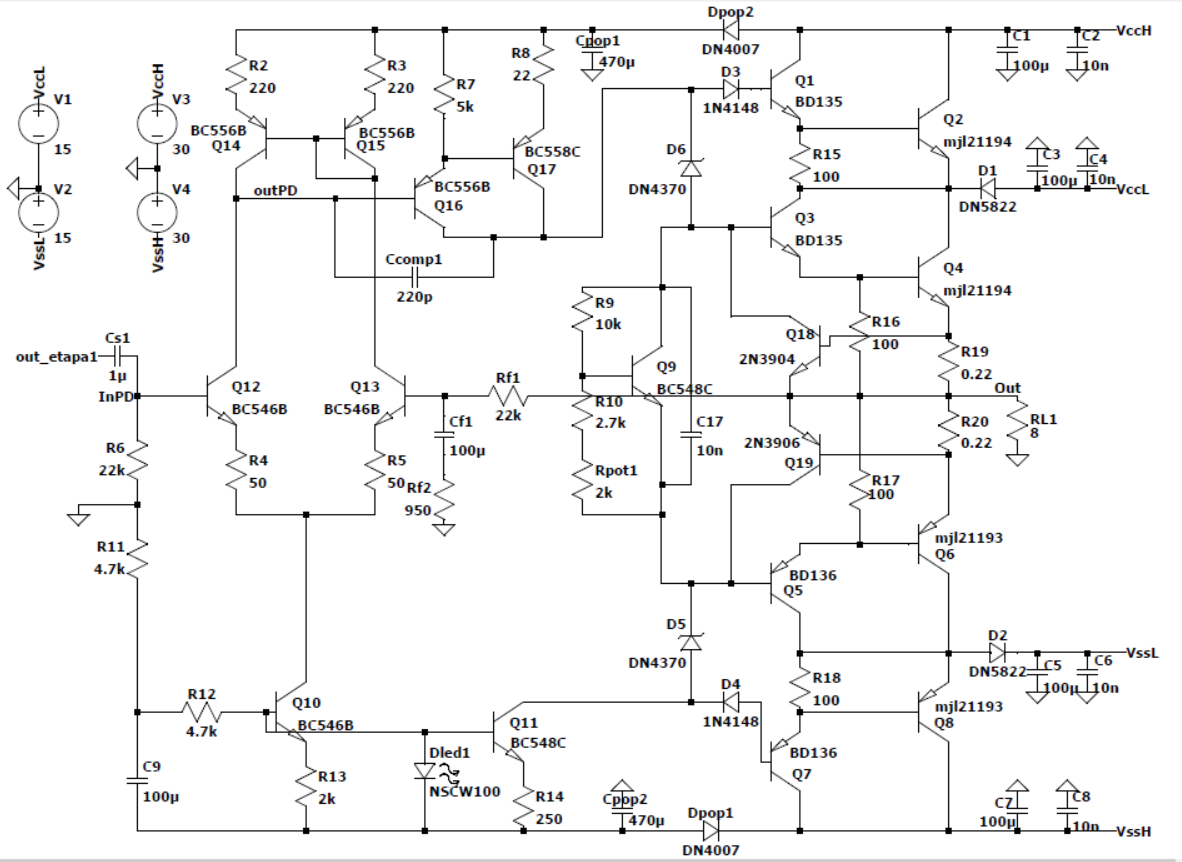
\includegraphics[scale=0.6]{./Amplificador_claseG.PNG}
        \caption{Esquemático de amplificador con clase G}
        \label{fig::Amplificador_claseG}
\end{figure}

\begin{figure}[H]
        \centering
        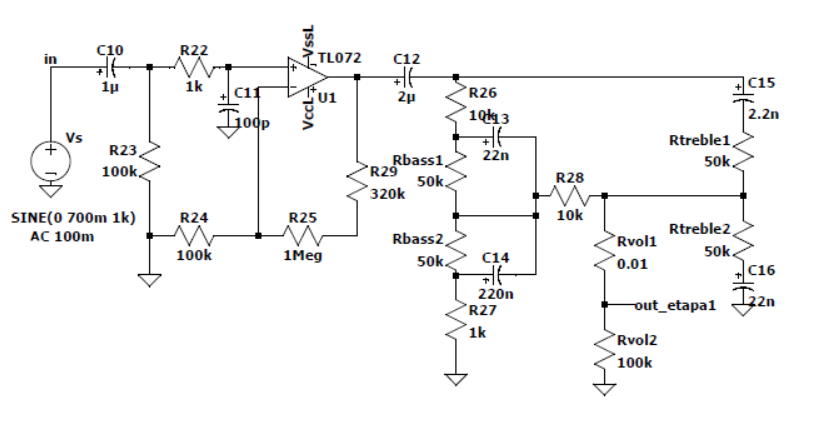
\includegraphics[scale=0.8]{./Pre_amplificador.PNG}
        \caption{Esquemático Pre-amplificador propuesto}
        \label{fig::Preamp}
\end{figure}

\begin{figure}[H]
        \centering
        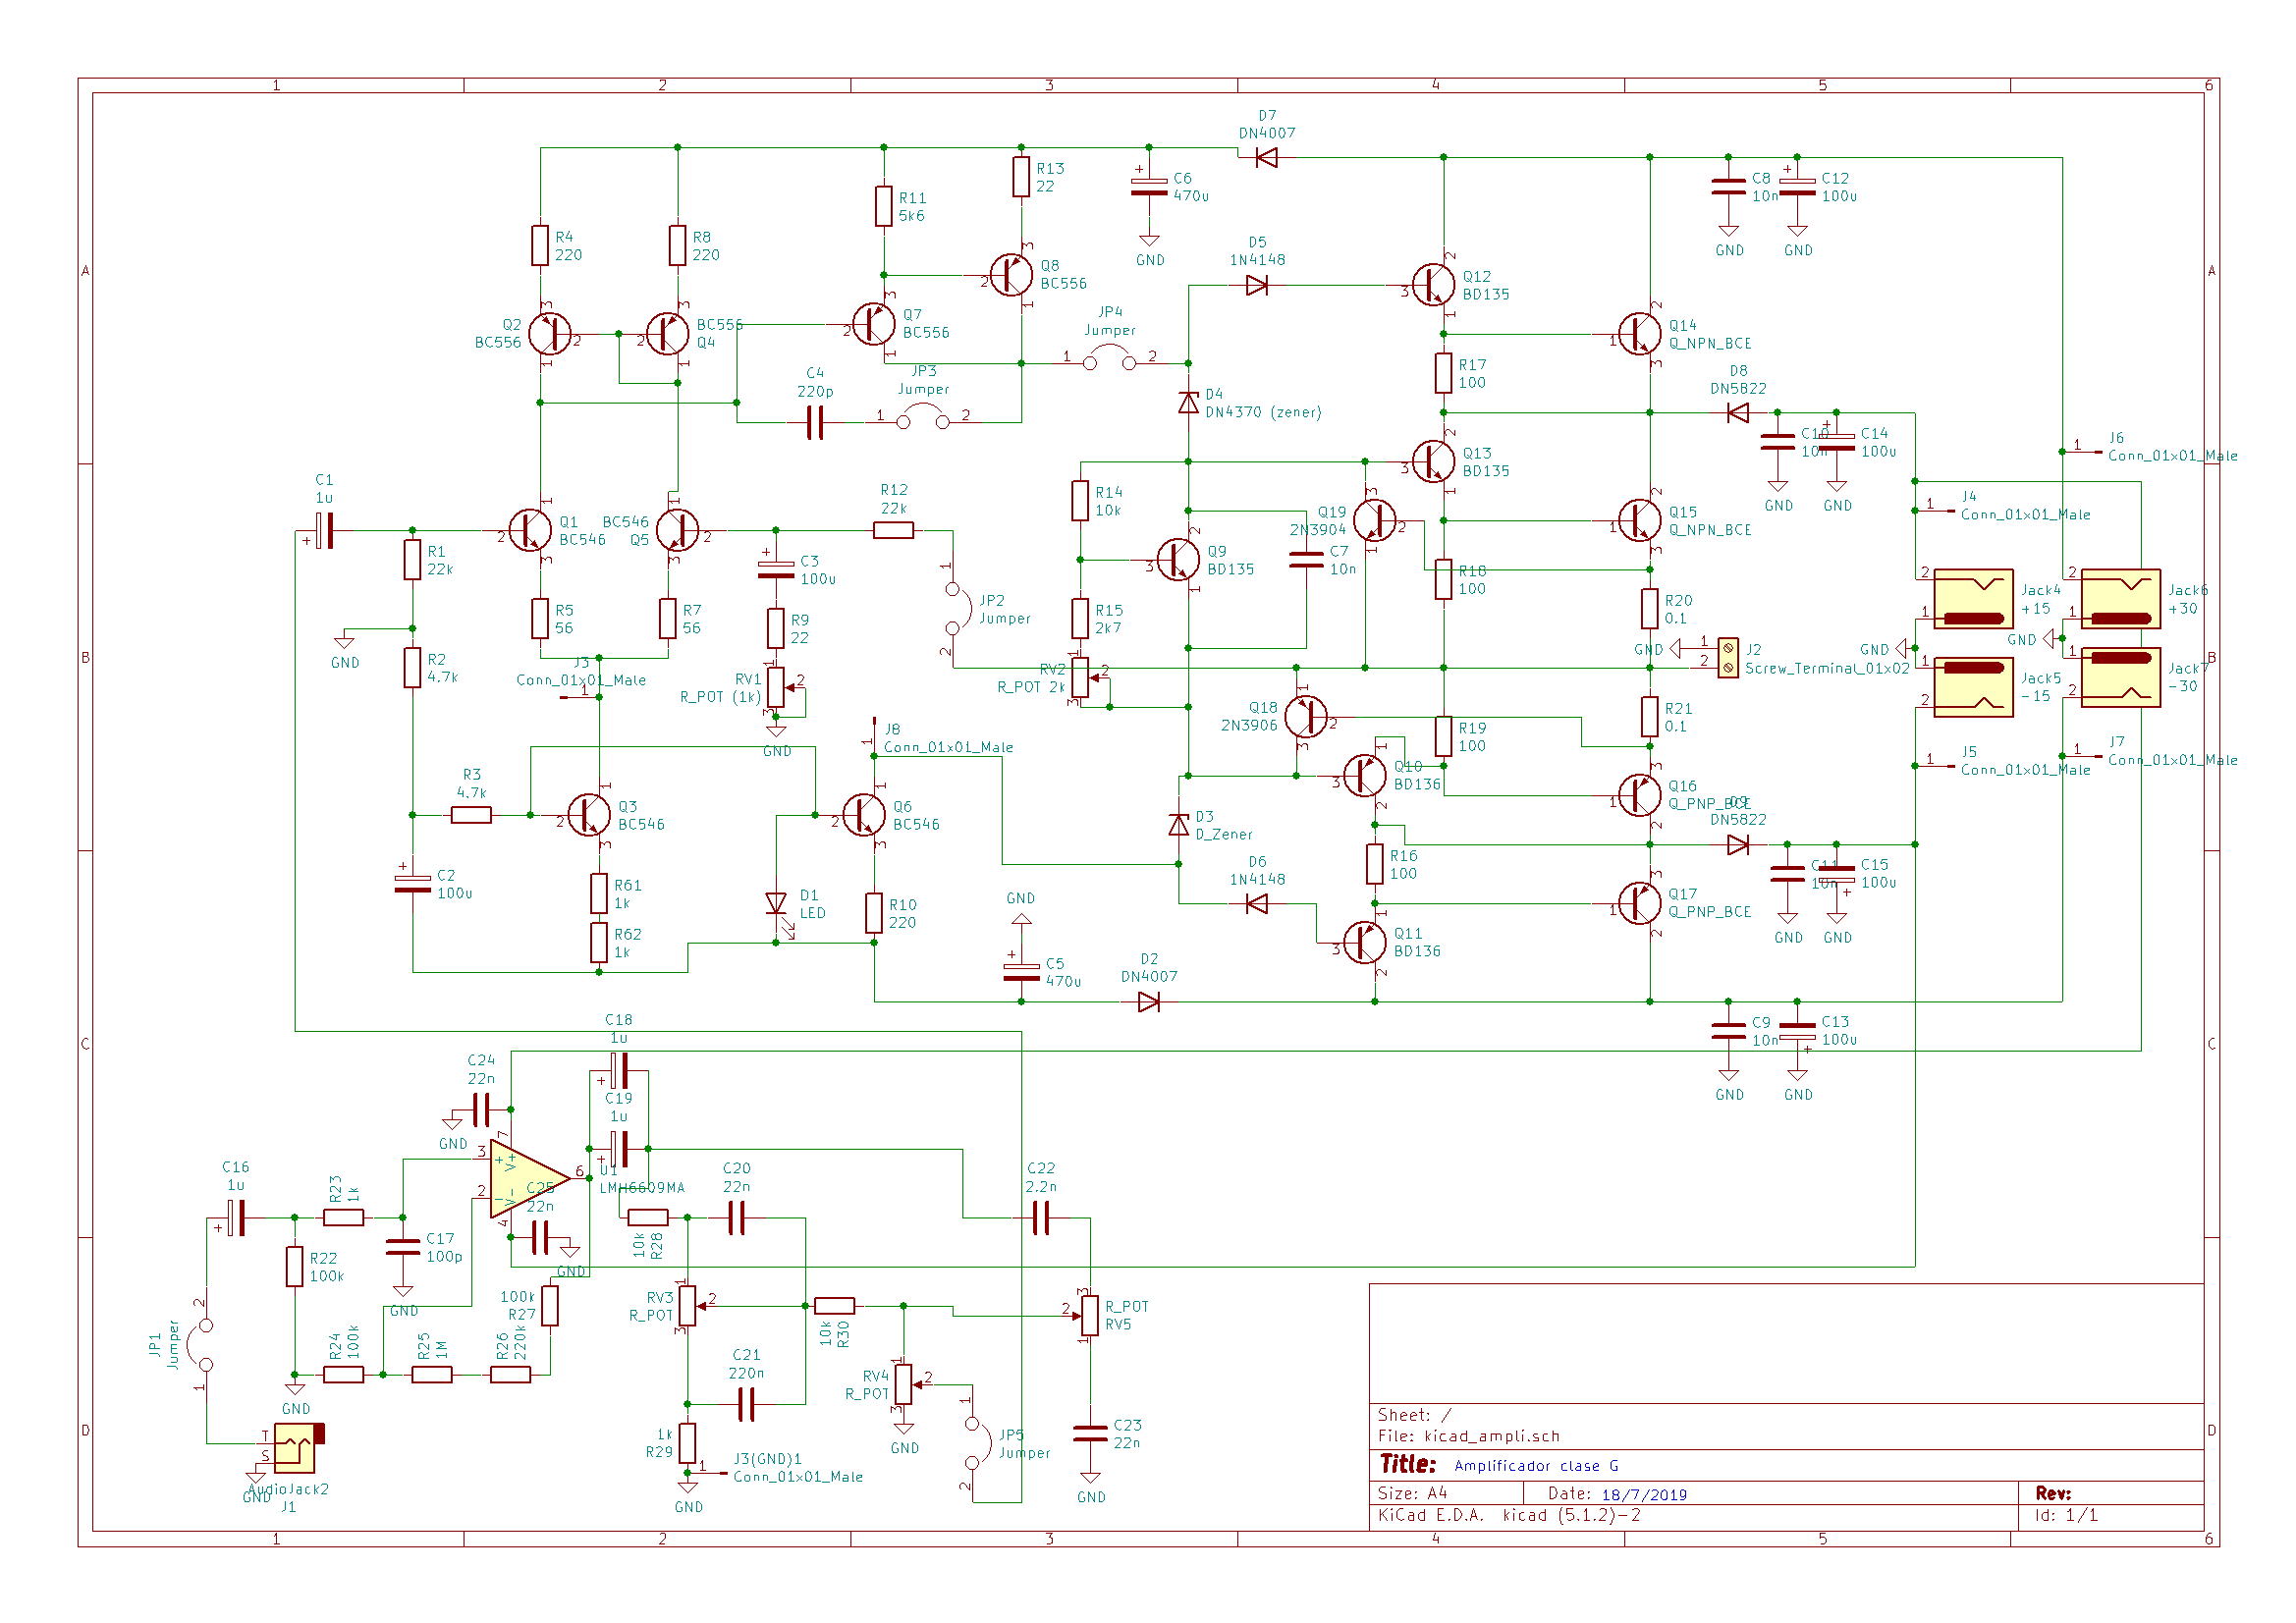
\includegraphics[scale=0.36]{./Amplificador_completo.png}
        \caption{Esquemático del circuito completo a implementar}
        \label{fig::Amplificador_completo}
\end{figure}

A continuación se muestran imágenes del PCB para el amplificador clase G a implementar:

\begin{figure}[H]
        \centering
        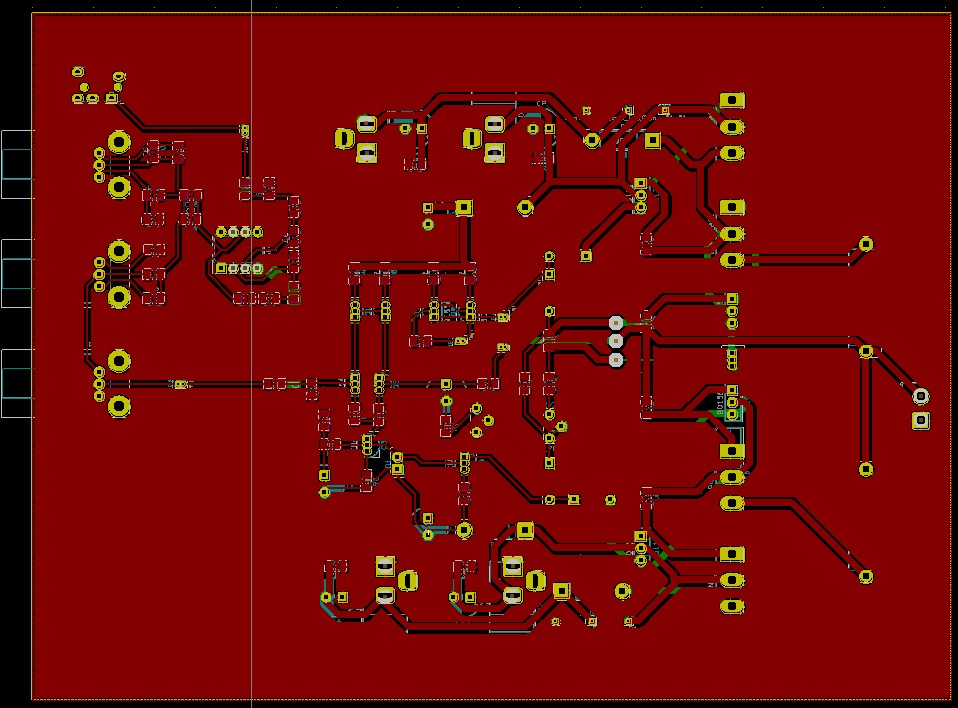
\includegraphics[scale=0.3]{./PCB1.jpeg}
        \caption{Vista de las pistas del PCB a implementar}
        \label{fig::PCB1}
\end{figure}

\begin{figure}[H]
        \centering
        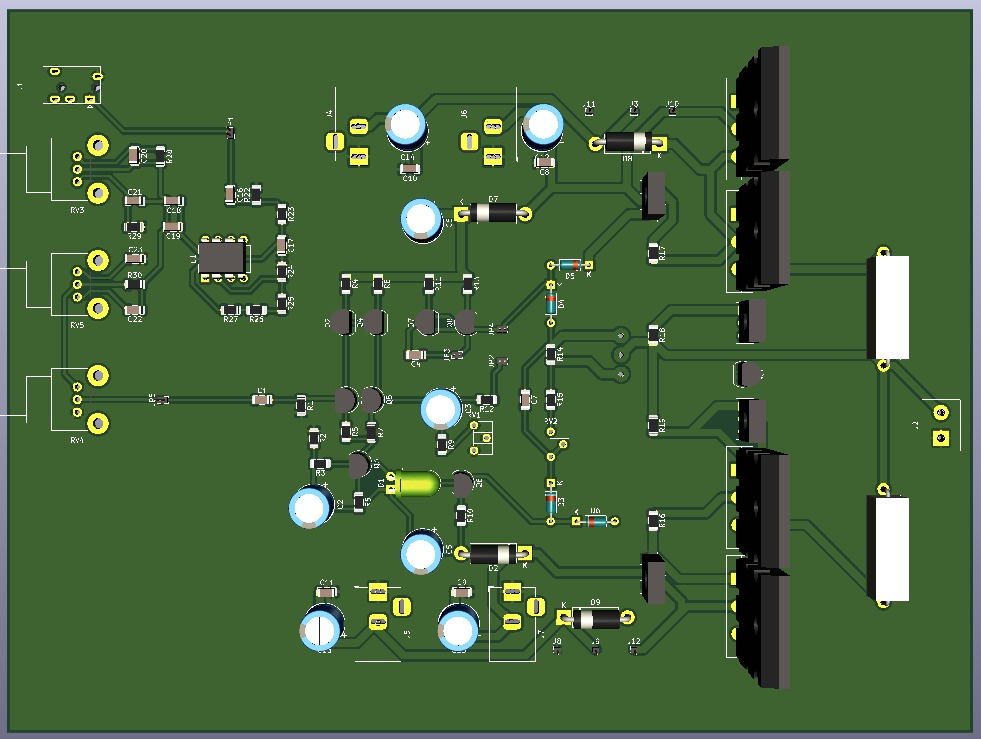
\includegraphics[scale=0.3]{./PCB2.jpeg}
        \caption{Vista superior del PCB a implementar}
        \label{fig::PCB2}
\end{figure}

A continuación se muestran imágenes del PCB para la fuente a implementar:

\begin{figure}[H]
        \centering
        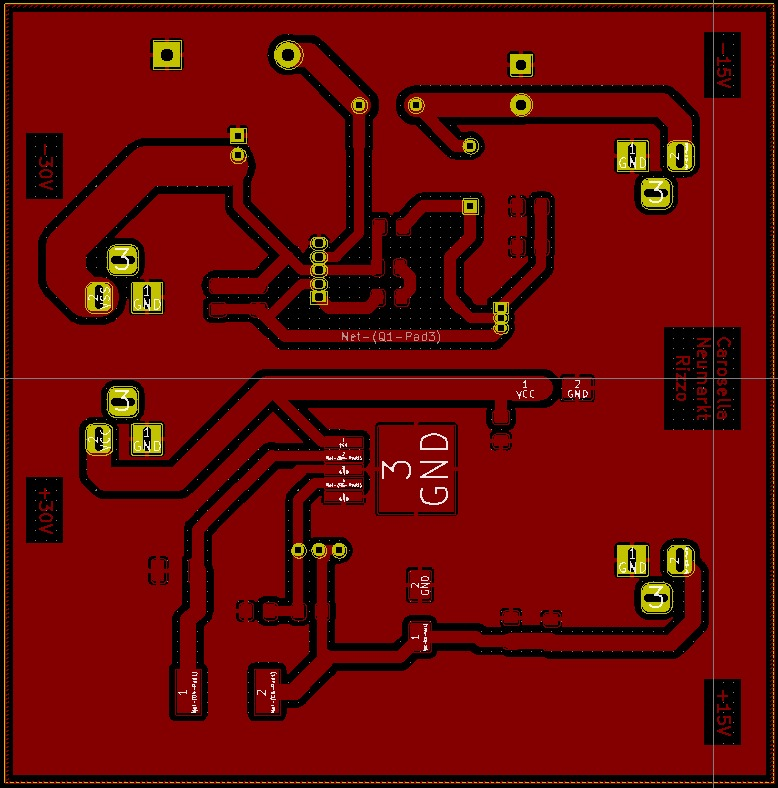
\includegraphics[scale=0.2]{./PCB_fuente1.jpeg}
        \caption{Vista de las pistas del PCB de la fuente a implementar}
        \label{fig::PCB1}
\end{figure}

\begin{figure}[H]
        \centering
        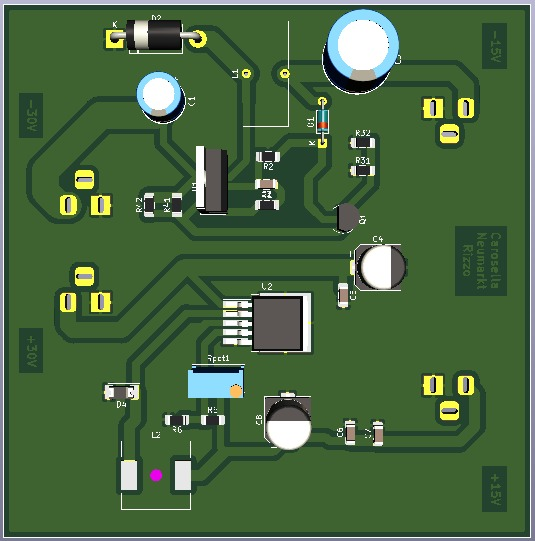
\includegraphics[scale=0.3]{./PCB_fuente2.jpeg}
        \caption{Vista superior del PCB de la fuente a implementar}
        \label{fig::PCB2}
\end{figure}


\par A continuación se muestra en el cuadro \ref{tab::lista_componentes} la lista de componentes a utilizar para la realización del amplificador clase G con sus respectivas especificaciones:\\

\begin{table}[]
\begin{tabular}{|l|l|c|c|c|c|c|}
 \hline
Componente   & Tipo              & Modelo   & Valor   & Tolerancia  & Potencia         & Tensión máx.       \\ \hline
R2            & película metálica & -        & 220\ohm       & 0.10\%      & \textless{}50uW  & -           \\ \hline
R3            & película metálica & -        & 220\ohm       & 0.10\%      & \textless{}50uW  & -           \\ \hline
R4            & película metálica & -        & 50\ohm        & 0.10\%      & \textless{}50uW  & -           \\ \hline
R5            & película metálica & -        & 50\ohm        & 0.10\%      & \textless{}50uW  & -           \\ \hline
R6            & película metálica & -        & 22k\ohm       & 0.1\%/0.5\% & \textless{}50uW  & -           \\ \hline
R7            & película metálica & -        & 5k\ohm        & 0.1\%/0.5\% & \textless{}300uW & -           \\ \hline
R8            & película metálica & -        & 22\ohm        & 0.1\%/0.5\% & \textless{}50mW  & -           \\ \hline
R9            & película metálica & -        & 10k\ohm       & 0.10\%      & \textless{}1mW   & -           \\ \hline
R10           & película metálica & -        & 2.7k\ohm      & 0.10\%      & \textless{}1mW   & -           \\ \hline
Rpot1         & Potenciómetro     & -        & 5k\ohm        & -           & \textless{}1mW   & -           \\ \hline
R11           & película metálica & -        & 4.7k\ohm      & 0.1\%/0.5\% & \textless{}170mW & -           \\ \hline
R12           & película metálica & -        & 4.7k\ohm      & 0.1\%/0.5\% & \textless{}170mW & -           \\ \hline
R13           & película metálica & -        & 2k\ohm        & 0.1\%/0.5\% & \textless{}5mW   & -           \\ \hline
R14           & película metálica & -        & 250\ohm       & 0.1\%/0.5\% & \textless{}80mW  & -           \\ \hline
R15           & película metálica & -        & 100\ohm       & 0.10\%      & \textless{}80mW  & -           \\ \hline
R16           & película metálica & -        & 100\ohm       & 0.10\%      & \textless{}80mW  & -           \\ \hline
R17           & película metálica & -        & 100\ohm       & 0.10\%      & \textless{}80mW  & -           \\ \hline
R18           & película metálica & -        & 100\ohm       & 0.10\%      & \textless{}80mW  & -           \\ \hline
R19           & alambre           & -        & 0.1\ohm       & 0.10\%      & 5W               & -           \\ \hline
R20           & alambre           & -        & 0.1\ohm       & 0.10\%      & 5W               & -           \\ \hline
RF1           & película metálica & -        & 22k\ohm       & 0.10\%      & \textless{}50mW  & -           \\ \hline
RF2           & película metálica & -        & 500\ohm       & 0.10\%      & \textless{}5mW   & -           \\ \hline
Rpot2         & Potenciómetro     & -        & 1k\ohm        & -           & -                & -           \\ \hline
Rcomp2        & película metálica & -        & 1\ohm         & 0.10\%      &                  & -           \\ \hline \hline
C1            & electrolítico     & -        & 100uF         &             & -                & \textless{}30V \\ \hline
C2            & cerámico          & -        & 10nF          &             & -                & \textless{}30V \\ \hline
C3            & electrolítico     & -        & 100uF         &             & -                & \textless{}15V \\ \hline
C4            & cerámico          & -        & 10nF          &             & -                & \textless{}15V \\ \hline
C5            & electrolítico     & -        & 100uF         &             & -                & \textless{}30V \\ \hline
C6            & cerámico          & -        & 10nF          &             & -                & \textless{}30V \\ \hline
C7            & electrolítico     & -        & 100uF         &             & -                & \textless{}15V \\ \hline
C8            & cerámico          & -        & 10nF          &             & -                & \textless{}15V \\ \hline
C9            & electrolítico     & -        & 100uF         &             & -                & \textless{}30V \\ \hline
Cs            & electrolítico     & -        & 1uF           &             & -                &                \\ \hline
Cf            & electrolítico     & -        & 100uF         &             & -                &                \\ \hline
Ccomp1        & cerámico          & -        & 220pF         &             & -                &                \\ \hline
Ccomp2        & cerámico          & -        & 10nF          &             & -                &                \\ \hline
Cpop1         & electrolítico     & -        & 470uF         &             & -                & \textless{}30V \\ \hline
Cpop2         & electrolítico     & -        & 470uF         &             & -                & \textless{}30V \\ \hline \hline
D1            & Schottky          & MBR1645  &               &             &                  &                \\ \hline
D2            & Schottky          & MBR1645  &               &             &                  &                \\ \hline
D3            & Silicon           & 1n4148   &               &             &                  &                \\ \hline
D4            & Silicon           & 1n4148   &               &             &                  &                \\ \hline
D5            & Zener             & N4370    &               &             &                  &                \\ \hline
D6            & Zener             & N4370    &               &             &                  &                \\ \hline
Dpop1         & Rectifier         & RR2L4s   &               &             &                  &                \\ \hline
Dpop2         & Rectifier         & RR2L4s   &               &             &                  &                \\ \hline
Dled          & Led               & NSCW100  &               &             &                  & \\ \hline 
\end{tabular}
\caption{Lista de componentes para el amplificador clase G}
\label{tab::lista_componentes}
\end{table}

\par Se optó para el proyecto realizar una etapa de salida clase G, a modo de cumplir con el requerimiento de realizar un proyecto que presente algún tipo de conmutación en el circuito. Basándonos en el libro \textit{AudioPower Amplifier Design Handbook} de Douglas Self, optamos por la realización de una arquitectura para el amplificador de 3 etapas:\\

\begin{itemize}
    \item 1) Etapa de entrada
    \item 2) Amplificación de tensión
    \item 3) Etapa de potencia a la salida
\end{itemize}

\par Para la etapa de entrada, se opto por aplicar un Par diferencial (PD) a n de obtener una entrada con mayor inmunidad al ruido posible (se aprovecha el alto rechazo al modo común de los pares diferenciales) y aprovechar la linealidad que tienen los pares diferenciales en comparación con las entradas con un solo transistor.\\

\par Aplicamos una carga activa para tener una ganancia mas grande que con una carga resistiva y que dependa de \textit{gm}. En las salida de los emisores NPN, se incluyeron resistencias pequeñas para mejorar la excursión y la linealidad e la etapa por medio de realimentación local. Las resistencias en los emisores PNP de la carga activa para mejorar la copia de corriente en las ramas del diferencial, además la resistencia R27 también se incluye para dicho n. Luego, se polariza el par diferencial con una fuente de corriente simple, a modo de independizar la polarización de la fuentes de alimentación (a diferencia de utilizar una resistencia, por ejemplo).\\

\par Luego, se incluye una compensacion dada por Ccomp2 y Rcomp2, ya que al analizar las simulaciones, se obtena una oscilacion en la se~nal de salida del PD.\\

\par Para la etapa de ganancia de tensión, se utilizo un par Darlington PNP a fin de obtener una buena ganancia de corriente en la etapa de amplificación. Se le agrega una compensación con Ccomp1, para mantener un buen margen de fase en el circuito ($MF = 62^\circ $).\\

\par En la etapa de salida se implemento un amplificador clase G. A n de obtener de una eficiencia mayor que en un clase B o AB, en la clase G se realiza una conmutación de las fuentes de alimentación a la salida según la señal lo amerita. En cuanto la señal de salida supera cierto umbral, se utilizan las fuentes de alimentación con mayor tensión, esto evita que ante señales de poco volumen se disipe un exceso de potencia innecesaria. La etapa fue implementada con transistores en modo Darlington, de este modo se obtiene una mejor ganancia de corriente a la salida y menor impedancia de salida.\\
%HOLI
\par Utilizamos un multiplicador de Vbe para polarizar los transistores. Observamos que se utilizan los diodos Zenner D5 y D7 para aprovechar la tensión fija del multiplicador de Vbe y mantener una diferencia de tensión entre las bases de los transistores de baja señal con los de alta señal, de modo que si la señal lo requiera, los transistores de alta señal ya estarán encendidos a tiempo antes de que los transistores de baja señal no tengan suficiente tensión de colector para la señal.\\

\par Por último, la inclusión de los diodos D1 y D2 se utiliza para que cuando la señal realice la conmutación y necesite mayor tensión de alimentación, las fuentes VccL y VssL queden sin efecto. Se utilizaron diodos Schottky para asegurar tiempo de acción rápida.\\

\par Se incluyeron capacitores cerca de las fuentes para filtrar ruidos de las mismas, y los diodos D9 y D8, con los capacitores C5 y C6 para evitar el ruido ``pop'' y ``click'' al encender y apagar el circuito.\\

\subsection{Polarización}

\par Se simularon los valores en reposo de los transistores de la etapa amplificadora clase G, junto con la máxima potencia disipada en cada uno. Los resultados se muestran en el cuadro \ref{tabla_reposo_calculo}:


\begin{table}[H]
\begin{center}
\begin{tabular}{llllll}
\hline\hline
Transistor & $V_{BQ}$ & $V_{CQ}$ & $V_{EQ}$ & $I_{CQ}$ & $P_{max}$\\
\hline \hline
Q1 (BD135) & 3.425V & 30V & 14.82V & 26.663pA & 120mW \\ 
Q2 (MJL21194) & 14.82V & 30V & 14.82V & 20.428pA & 7W \\ 
Q3 (BD135) & 1.189V & 14.82V & 529.91mV & 5.342mA & 1W \\ 
Q4 (MJL21194) & 529.91mV & 14.81V & -167.67uV & 2.63mA & 3W  \\ 
Q5 (BD136) & -1.217V & -14.82V & -522.78mV & -5.221mA & 1W \\ 
Q6 (MJL21193) & -522.78mV & -14.82V & -721.07uV & -2806mA & 3W \\ 
Q7 (BD136) & -3.453V & -30V & -14.82V & -26.634pA & 120mW \\ 
Q8 (MJL21193) & -14.82V & -30V & -14.82V & -17.52pA & 7W \\ 
Q9 (BC548C) & -516.2mV & 1.189V & -1.217V & 9.05mA & 22mW \\ 
Q10 (BC546B) & -26.3V & -676.53mV & -26.93V & 1.186mA & 32mW \\ 
Q11 (BC546B) & -26.3V & -3.45V & -26.93V & 9.25mA &223mW \\ 
Q12 (BC546B) & -31.67mV & 27.89V & -646.88mV & 591.557uA & 17mW \\ 
Q13 (BC546B) & -31.86mV & 28.58V & -646.88mV & 591uA & 17mW \\
Q14 (BC556B) & 28.58V & 28.58V & 29.19V & -591.29uA & 0.8mW \\ 
Q15 (BC556B) & 28.58V & 25.58V & 29.19V & -588uA & 0.4mW \\ 
Q16 (BC556B) & 27.88V & 3.42V & 28.45V & -186.64uA & 4.7mW \\ 
Q17 (BC556B) & 28.45V & 3.42V & 29.12V & -9.065mA & 236mW \\ 
Q18 (2N3904) & -167.67uV & 1-19V & -445.12uV & 1.203pA & 10pW \\ 
Q19 (2N3906) & -721.07uV & -1.22V & -445.12uV & -1.228pA & 10pW \\ \hline\hline
\end{tabular}
\caption{Punto de reposo de los transistores y máxima potencia disipada en operación}
\label{tabla_reposo_calculo}
\end{center}
\end{table}

\par Se verifico la corriente del amplificador operacional U1 (TL072), siendo la corriente que consume de $14.19mA$, consumiendo $425.83mW$. También se midieron las fuentes V1 (-22.17mA, -332.5mW), V2 (-22.21mA, -333.33mW), V3 (-10.44mA, -313.04mW) y V4 (-13.23mA, 396.95mW).

\subsection{Primera prueba con señal}

\par Se realizaron las primeras pruebas con señal al circuito completo.\\

\par Para una señal de $V_s = 0.8V$, $Rvol1 =2k\ohm$, $Rvol2 = 98k\ohm$, se produce el recorte notorio por saturación para una señal senoidal sin carga, con una tensión máxima $V_{out} = 25.32V$.

Para una señal de $V_s = 0.8V$, $Rvol1 =3k\ohm$, $Rvol2 = 97k\ohm$, se produce el recorte notorio por saturación para una señal senoidal con carga $RL=8\ohm$ a la salida, con una tensión máxima $V_{out} = 24.528V$ (Con $35.035W$ sobre $RL$).\\

\par Se repiten las mediciones pero con una señal cuadrada de $1kHz$ de frecuencia. Para una señal de $V_s = 0.8V$, $Rvol1 =1\ohm$, $Rvol2 = 100k\ohm$, se produce el recorte notorio por saturación para una señal cuadrada sin carga, con una tensión pico $V_{out} = 25.31V$.

Para una señal de $V_s = 0.8V$, $Rvol1 =1\ohm$, $Rvol2 = 100k\ohm$, se produce el recorte notorio por saturación para una señal cuadrada con carga $RL=8\ohm$ a la salida, con una tensión pico a la salida $V_{out} = 24.538V$ (Con $43.411W$ sobre $RL$).

Para las señales cuadradas se verifico que la salida no presente oscilaciones, amortiguamientos ni sobre-impulsos como se puede apreciar en la figura \ref{fig::Cuadrada_a1khz}.\\

\begin{figure}[H]
        \centering
        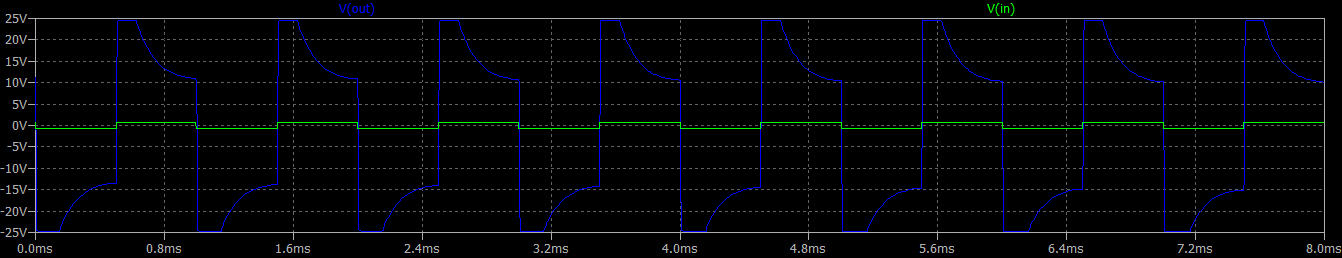
\includegraphics[scale=0.5]{./Cuadrada_a1khz.png}
        \caption{Señal cuadrada aplicada de 1kHz de frecuencia}
        \label{fig::Cuadrada_a1khz}
\end{figure}


\subsection{Ganancias}

\par Para el calculo de las ganancias, aplicamos a la entrada una tensión senoidal tal que a la salida se produce una tensión del $90\%$ a la que se produce el recorte, es decir, de acuerdo a lo calculado previamente $V_{out} = 22.08V$.

Para esto, aplicamos al circuito completo una tensión $V_s = 0.7V (1kHz)$ ($Rvol1 = 1.5k$, $Rvol2 = 98.5k$), obteniéndose a la salida una tensión $V_{out}==22.1572V$, es decir, se obtiene una ganancia de tensión de $A = 23.968 \frac{V}{V}$.

Repetimos la medición para una tensión 10 veces menor a la anterior, es decir, queremos que $V_{out} = 2.208V$. Las condiciones fueron, $V_s = 0.7V (1kHz)$ ($Rvol1 = 91k$, $Rvol2 = 9k$), obteniéndose a la salida una tensión $V_{out}= 2.0885V$, es decir, se obtiene una ganancia de tensión de $A = 24.18\frac{V}{V}$.\\

\par Por lo tanto, podemos verificar que no hay cambios significativos en la ganancia de corriente sobre el rango de tensiones de entrada de trabajo. En la figura \ref{fig::Max_tension_sobre_RL} se puede observar la máxima tensión nominal, sin recorte, sobre la carga.

\begin{figure}[H]
        \centering
        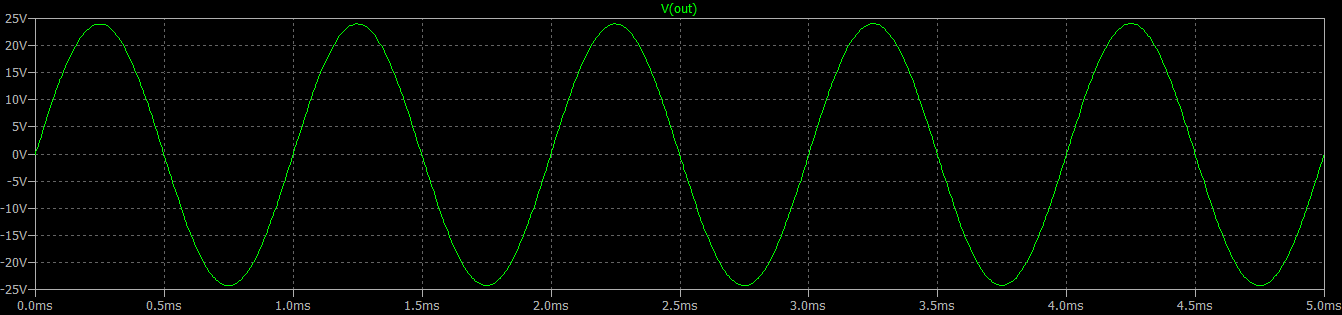
\includegraphics[scale=0.5]{./Max_tension_sobre_RL.png}
        \caption{Máxima tensión sin recorte sobre la carga $RL$}
        \label{fig::Max_tension_sobre_RL}
\end{figure}

\par Para constatar con lo medido, podemos observar que la ganancia $f$ del realimentador, teóricamente es $f = \frac{950\ohm}{950\ohm+22k\ohm} = 1/24.158\frac{V}{V}$. Considerando la expresión de la ganancia total realimentada $A = \frac{a}{1+af} \approx 1/f = 24.158\frac{V}{V} $\\

\par Luego, verificamos el valor de la ganancia de lazo "$af$", cortando el lazo de realimentación y cortocircuitando la entrada del amplificador "$a$". Se obtuvo un valor de $af = 230.22$, la cuál es mucho mayor a 1, por lo tanto aproximar la ganancia total por $1/f$ es correcto.

\subsection{Sensibilidad}

\par Medimos el valor eficaz de una señal senoidal de 1kHz aplicada a la entrada ($Vin (RMS)=693.82mV$ con $V_s = 0.7V$ a $1kHz$, $Rvol1 = 1\ohm$ y $Rvol2 = 100k\ohm$), que produce la potencia especificada a la salida con carga nominal, siendo esta última $V_{out}(RMS)= 16.742V$. \\


\subsection{Potencia de salida}

\par Se obtiene a la salida la mayor amplitud posible sin recorte a $1kHz$ y se mide $V_{out}=23.567V$. Se calcula la potencia disipada como se pide en el enunciado como: $P = \frac{V_{out}^2}{RL} = 69.43W$ ($35.035W$ RMS). También se midió la potencia de las fuentes de alimentación de $30V$, siendo esta $-24.126W$, a $804mA$ de consumo, y la alimentación de $15V$, con $-2.43W$ a $161.63mA$ de consumo.

\par Se repitió lo mismo pero utilizando una onda cuadrada de $1kHz$, obteniéndose $V_{out} = 24.53V$, por lo tanto $P = 75.21W$ ($19.485W$ RMS), siendo la potencia entregada por la fuente de alimentación de $30V$, de $-8.905W$ a $296.83mA$ de consumo.

\subsection{Ancho de banda}

\par Se calcula el ancho de banda solo del amplificador clase G, ya que el preamplificador tiene un procesamiento de la señal en la cuál afecta los graves y agudos.

\par Se puede observar en la figura \ref{fig::Rta_frec_baja_potencia}, la respuesta en frecuencia a baja frecuencia. Esto sería a una tensión $V_{out}= 2.41$ ($Vin = 100mV$, la misma se considera como 10\% de la máxima especificada). A estas condiciones, se obtiene un ancho de banda tal que la frecuencia de corte inferior es $fi = 7.62Hz$ y la frecuencia de corte superior $fh = 203.7kHz$, con una ganancia de magnitud $7.65dB$.\\ 

\begin{figure}[H]
        \centering
        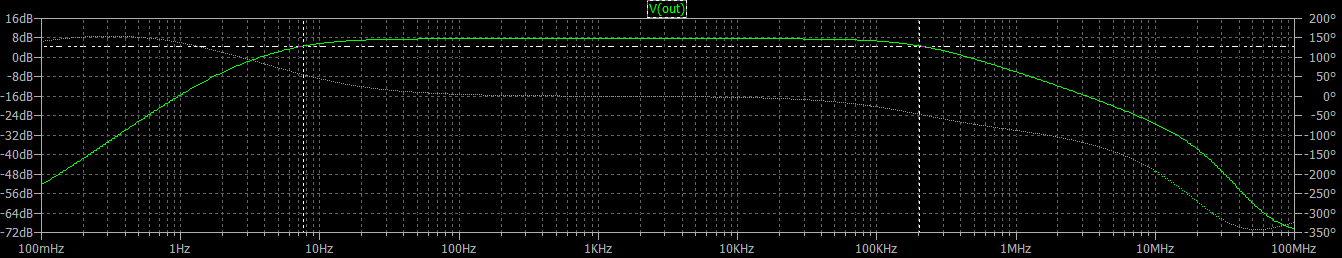
\includegraphics[scale=0.5]{./Rta_frec_baja_potencia.png}
        \caption{Respuesta en frecuencia a baja potencia}
        \label{fig::Rta_frec_baja_potencia}
\end{figure}

\par Se repite el cálculo para una señal de alta potencia ($V_{out} = 24.03V$, $Vin = 1V$), obteniéndose la figura \ref{fig::Rta_frec}. El ancho de banda de la señal a estas condiciones fue $fi = 6.65Hz$, $fh = 233.88kHz$ y una ganancia de magnitud $27.65dB$.

\begin{figure}[H]
        \centering
        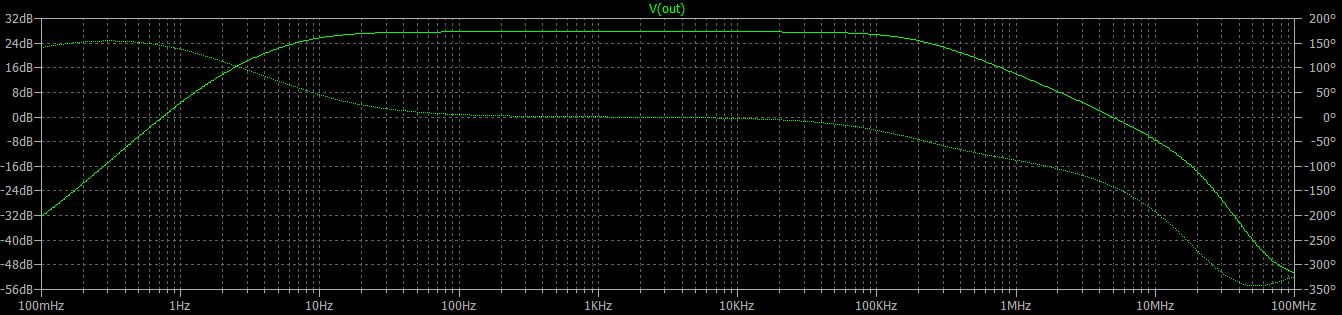
\includegraphics[scale=0.5]{./Rta_frec.png}
        \caption{Respuesta en frecuencia a alta potencia}
        \label{fig::Rta_frec}
\end{figure}

\subsection{Slew Rate}



\par Se aplicó una cuadrada a modo de obtener el valor numérico del SR, calculando la pendiente de la recta obtenida en la figura \ref{fig::Slew_rate_escalon}. A partir del gráfico, se obtuvo un valor de $SR = 5.167 V /\mu seg$ lo que implica un ancho de banda de potencia de $f_{PBW} = 33.5kHz$. También puede observarse un pico en la recta, el cuál se debe a la conmutación de las fuentes de salida.

\begin{figure}[H]
        \centering
        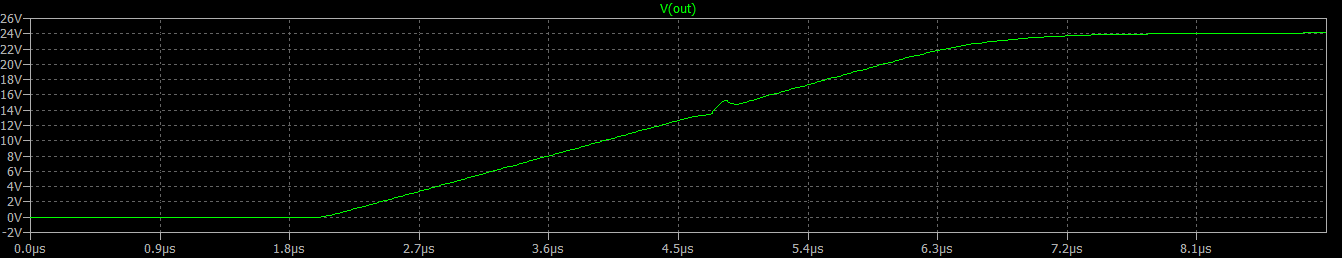
\includegraphics[scale=0.5]{./Slew_rate_escalon.png}
        \caption{Escalón aplicado a la señal para medir el SR}
        \label{fig::Slew_rate_escalon}
\end{figure}


\subsection{Impedancia de entrada}

\par Para el cálculo de la impedancia de entrada del amplificador, se procedió colocando una señal de $Vin = 500mV$ a $1kHz$ en la entrada del amplificador clase G(sin el pre-amplificador) y se varío un resistor en serie con la fuente de señal a modo de obtenerse una señal 50\% menor a la aplicada $Vin$. Se obtuvo a $Vin_{amplificador} = 256mV$ que la impedancia de entrada era $Z_i = 21k\ohm$.

\par Se procedió de la misma manera variando la frecuencia de $100Hz$ a $10kHz$, obteniéndose el mismo valor de impedancia de entrada.\\

\par También se hizo lo mismo con la etapa pre-amplificadora, obteniéndose una impedancia de entrada de $Z_in =100k\ohm$. \\

\subsection{Impedancia de salida}

\par Para medir la impedancia de salida, se midió la tensión de salida con y sin carga $RL$, a una entrada $Vs = 0.7V$ ($Rvol1 = 1\ohm$ y $Rvol2 = 100k\ohm$), obteniéndose $V_{outS/C} = 23.5894V$ y $V_{outC/C = 23.644062V}$. Mediante el cálculo $Z_o = RL (\frac{V_{S/C}}{V_{C/C}}-1)$, se obtuvo $Z_o = 0.0185\ohm$.\\

\subsection{Factor de amortiguamiento}

\par Se calcula el factor de amortiguameniento como $\frac{RL}{Z_o} = 431.55$.

\subsection{Distorsión armónica y por intermodulación}

\par A un $1kHz$ de frecuencia, utilizando la directiva \textit{.FOUR} del LTspice, se obtuvo una distorsión armónica del $0.014348\%$.

\par Para definir la distorsión por intermodulación, se define en primer lugar un tono puro de baja frecuencia de $100Hz$ y luego otro tono de alta frecuencia de $5kHz$, y se aplica la suma a la entrada del amplificador, a una relación de amplitudes de 4 a 1 entre ambas fuentes. Luego se observa el espectro de frecuencias a la salida y se calcula la IMD como la suma cuadrática de las amplitudes de los subtonos alrededor de $5kHz$ y se lo divide por la amplitud del mismo. Se determina la IMD para potencias de $0.1W$, $1W$, $10W$ y $90\%$ de la potencia máxima:


\begin{table}[H]
\centering
\begin{tabular}{llll}
\hline\hline
Potencia $[W]$ & $V_{o_P}$ $[V]$ & $V_{i_P}$ $[mV]$ & IMD [\%]  \\\hline\hline
0.1     & 1.789      & 74.53         & 0.08062 \\
1       & 5.65      & 236        & 0.09642\\
10      & 17.88     & 745        & 0.06937\\
19.19   & 21.21     & 883        & 0.1\\
\hline \hline
\end{tabular}
\end{table}

\subsection{Estabilidad y Margen de fase}

\par Se obtuvo un sistema estable midiendo el margen de fase de la ganancia de lazo. Se obtuvo un margen de fase de $MF = 79.2^\circ$ a $150kHz$ como se puede apreciar en la figura \ref{fig::Estabilidad_MF}.

\begin{figure}[H]
        \centering
        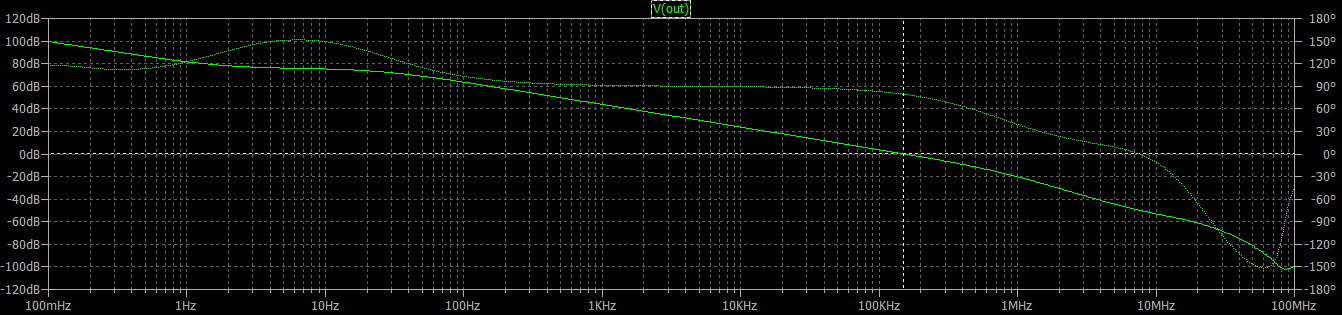
\includegraphics[scale=0.5]{./Estabilidad_MF.png}
        \caption{Respuesta en frecuencia de la ganancia de lazo para la estabilidad}
        \label{fig::Estabilidad_MF}
\end{figure}

\subsection{Cálculo de disipadores}

\par Para el cálculo de disipadores, se consideró el peor caso en el cuál los transistores disipan la mayor potencia posible. Esto es crítico en el caso de los transistores de potencia de salida cuando se trabaja en con la alimentación más alta. Para ese caso, sabemos por los datos de los datasheet de todos los transistores en la salida que la resistencia térmica de los transistores es de $R_{j-c} = 0.7^\circ C/W$. Considerando que se acoplan térmicamente los 4 en el mismo disipador más el multiplicador de $V_{be}$ y los drivers internos que conforman la malla de control de embalamiento, se puede utilizar la analogía circuital de modelos en paralelo para los cálculos de disipación. Medimos que para los transistores Q2 y Q8, la máxima potencia disipada es $7W$, para $Q4$ y $Q6$ es $3W$, mientras que la suma de $Q3$, $Q5$ y $Q9$ no supera los $250mW$ (lo cuál está considerado en las potencias de 7W y 3W). Esta condición se da para $0.64 V_{cc} = 0.64 \cdot 30V = 19.2V$. Sin embargo, se verificó por simulación y el peor caso se da para $Vin = 0.9V$. Finalmente la temperatura máxima de los transistores es de $150^\circ C$ la cuál se multiplica por un factor de seguridad del 80\%, y se considera una temperatura ambiente de $40^\circ C$ nuevamente por cuestiones de seguridad. Se tiene que el disipador debe tener la siguiente resistencia térmica:

\begin{equation}
    R_{d-a} = \frac{0.8 \cdot 150^\circ C-40^\circ C}{(7W+3W) \cdot 2} - \frac{0.7^\circ C/W}{2} - \frac{1^\circ C/W}{2} = 3.15^\circ C/W
\end{equation}

Por lo tanto, se considera que los disipadores necesarios para el circuito pueden ser $ZD6$, $ZD7$, $ZD8$, $ZD16$, $ZD28$ ó $ZD30$, cuyas resistencias térmicas son $2.9^\circ C/W$, $2.6^\circ C/W$, $2.9^\circ C/W$, $2.2^\circ C/W$, $2.9^\circ C/W$, $2.4^\circ C/W$ respectivamente.


\subsection{Verificación de embalamiento térmico}

\par Utilizando la fórmula vista en clase y considerando $R_{j-a}Q1 = 10^\circ C/W$, $B_{min} = 8$ se calcula:

\begin{equation}
    R_E > \frac{R_{j-a}Q1 \cdot Vcc \cdot K}{(B_{min}+1)} = \frac{10^\circ C/W \cdot 30V \cdot 2}{(8+1)} = 0.0333\ohm 
\end{equation}

Por lo tanto, se verifica que el valor de $R_E = 0.1\ohm$ es correcto.